\documentclass{article}
\usepackage{graphicx}
\graphicspath{ {images/} }


\newcommand{\tab}[1]{\hspace{.1\textwidth}\rlap{#1}}

\begin{document}
	
\begin{titlepage}
	\newcommand{\HRule}{\rule{\linewidth}{0.5mm}} % Defines a new command for the horizontal lines, change thickness here

	\center % Center everything on the page
	 
	%----------------------------------------------------------------------------------------
	%	LOGO SECTIONS
	%----------------------------------------------------------------------------------------

	\includegraphics[width=\textwidth]{front-page}

	%----------------------------------------------------------------------------------------
	%	TITLE SECTION
	%----------------------------------------------------------------------------------------

	\HRule \\[0.4cm]
	{ \huge \bfseries Software Requirements Specification}\\[0.4cm] % Title of your document
	\HRule \\[1.5cm]
	 
	%----------------------------------------------------------------------------------------
	%	MEMBERS, TEAM NAME SECTION
	%----------------------------------------------------------------------------------------

	\begin{minipage}{0.5\textwidth}
	\begin{flushleft} \large
	\emph{Members:}\\% add your name and student here
	Peter Boxall 14056136	
	
	Orisha Orrie 13025199
	
	Nsovo Baloyi 12163262
	
	Elizabeth Bode 14310156
		
	Robert Trankle 15092454

	Nikki Constancon 15011713

	Ernst Eksteen 28398603
	\end{flushleft}
	\end{minipage}
	~
	\begin{minipage}{0.4\textwidth}
	\begin{flushright} \large
	{ \huge \bfseries Team Fuchsia }% Title of document
	{\large \today}\\
	{\large v0.1}
	\end{flushright}
	\end{minipage}\\[4cm]
\end{titlepage}


	\newpage
	
	\section{Introduction}
    	
        \subsection{Purpose}
        	\paragraph{The purpose of this document is to put forth a description detailing the NavUP system. It will explain the main purpose of the system, as well as additional subsystems, the interface of these systems, and what they will and will not do, as well as the constraints. Providing a detailed requirement specification of the system as a whole. It is intended for the Client, as well as developers who will integrate the system.}
    	\subsection{Scope}
        	\paragraph{NavUP will be a mobile device application, that will provide the basic functionalities of a navigation system. The system will only interoperate and function on the Hatfield main campus of the University of Pretoria.  	NavUp will provide a means to navigate the main campus of the University of Pretoria. It will thus provide users choices with regards to which routes they wish to take to reach there destination, taking into account factors such as pedestrian and vehicle traffic as well as providing routes that cater to users who may suffer physical disabilities.  NavUP's goal is to provide a personalised, efficient and convenient means of traversing the university's Hatfield campus. The system will also provide extra additional information regarding useful points of interests such as bathroom locations, as well as provide information to the user regarding the rich history of the University of Pretoria. The navigation system will be required to constantly be connected the the campus's WI-FI and will continually send up and down stream information to a server with regards to users location and destination. The server will be required to calculate the route and factor in additional information as set up by the user and there needs. The server must also be able to handle a high volume of concurrent users and provide them all with there required data. Location tracking will be achieved through the use of --WI-FI signal strength and other : not sure of exact methodology-- techniques and not through the use of GPS. /* This means that the two way communication between the device and the server must --explain requirements here-- */ }
        \subsection{Definitions, Acronyms, and Abbreviations}
        \subsection{References}
        \subsection{Overview}
	
	\section{Overall Description}
		
        \subsection{Product Perspective}
        
        	\subsubsection{System Interface}
            \subsubsection{User Interface}
	    {All users will have access to the navigation system when the application is launched.
They will be able to enter a destination and follow the path to location/lecture hall specified(see Figure 1).
The users will also be able to select preferences such as disability access path, which will enable them to travel the path with ease.\\\\
The users will be able to view information each building, giving them additional historic information about the building(Figure 2). If they do not not wish to 
view information about the building, they must simply not click on the information symbol available.
They will also be allowed to view each room. The navigation system will allow the users to select points of interest, such as food dispensaries, 
smoking locations, and toilets. They will be able to turn on and off indicators for these points of interest.
The users may access a view to heat paths on the map, to show an increase in crowd population in a dense area.\\\\
For the account user interface, the registered students and employees will be able to login to their account, using their clickUP information.
There will be certain accounts with administrative privileges that will be able to create and delete accounts, as deemed necessary.\\\\
The application will be able to send users notifications, on events that occur on campus as well as a report of information, such as the amount of 
steps walked per week. Students and employees will be able to remove push notifications, if they do not wish to receive them from the system.\\\\
}
\begin{figure}[h]
\centering
\begin{minipage}{.5\textwidth}
	\centering
	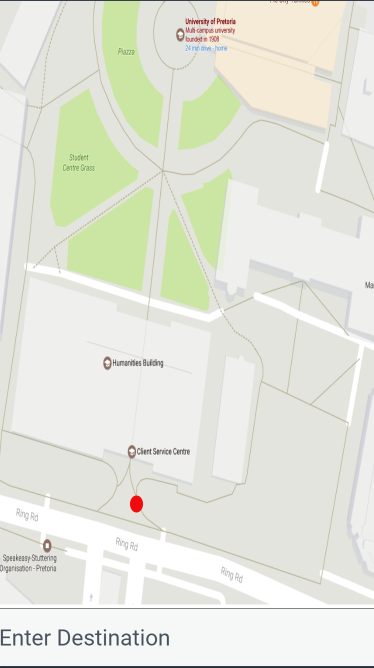
\includegraphics[width=2cm, height 8cm]{Navigation}
	\caption{Navigation System}
\end{minipage}%
\begin{minipage}{.5\textwidth}
	\centering
	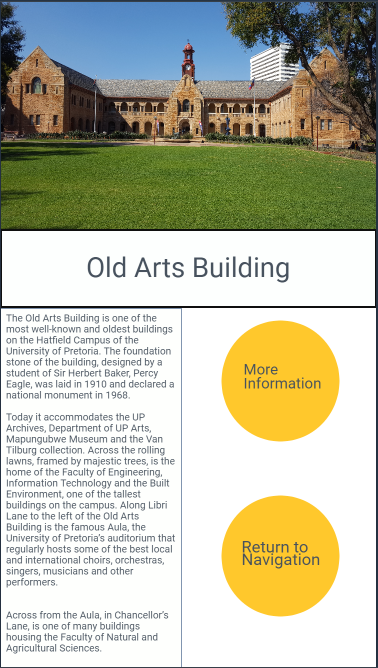
\includegraphics[width=2cm, height 8cm]{BuildingInfo}
	\caption{Building Information}
\end{minipage}%
\end{figure}


            \subsubsection{Hardware Interface}
		\paragraph{

			

			Wifi will The hardware intefaces used by the aplication will 

			The op systems of the phnes abstarct certin interfaces like the wifi and the gps so you dont have to

Since neither the mobile application nor the web portal have any designated hardware, it does not have 
any direct hardware interfaces. The physical GPS is managed by the GPS application in the mobile phone 
and the hard
ware connection to the database server is managed by the underlying operating system on the 
m
obile phone and the web server

}
            \subsubsection{Software Interface}
            \subsubsection{Communications Interface}
            \subsubsection{Memory}
            \subsubsection{Operations}
            \subsubsection{Sit Adaption Requirements}
        
		\subsection{Product Functions} \paragraph{The main function of the NavUP system will be to show students how to get around campus in the shortest possible way. Thus, this will entail using WiFi, mobile networks and possibly GPS to navigate around Hatfield campus. The basic functions will include:  }
	\begin{itemize}
  		\item A heat map to show pedestrian traffic.
		\item Providing the shortest path from point A to point B.
 		 \item A distance tracker to show users the distance left until they reach their destination.
		\item A specialized route for disabled users.
		\item Points of interest around the university such as restaurants, ATMs, the church, Scienza and Botanical Gardens.
 		 \item Essential Areas such as bathrooms, parking areas and smoking areas.
		\item Exact locations of buildings as well as the lecture halls that they consist of.
		\item A "Where am I?" function to show users exactly what is around them.
 		 \item Historical backgrounds of buildings and different parts of campus.
		\item A login page for users who would like access to more of the personalised functions. Theses functions will be saving locations for future use, a game which rewards users when they reach a certain distance and saving user preferences and interests.
		\item A random facts generator for distance rewards.
		\item Switching between WiFi, mobile data and GPS to navigate around campus.
		\item A timetable function for users to input their timetables and show exactly where their lectures will take place with reminders.
		\item Provide adminitrative security for login functionality.
		\item Rating system and review for restaurants and parking.
		\item Route options such as scenic routes and fastest route.
		\item Ability to share directions as well as estimated time of arrival.
	\end{itemize}
    	\subsection{User Characteristics}  
		\paragraph{ 

There will be three main types of users interacting with the system, namely a general user, a registered user and an admin. Each of these types will have different rights and access to the system and thus their own requirements.

The general user will use the system to navigate from their location to another specified location. They will need minimal skill in order to utilise the application, including the ability to connect to the Wi-Fi and indicate intended location. The general user wll have restricted usage of the in-app game and certain privilages that require a user profile. They will ot require any additional expertise or education to function the application.

The registered user will have the same access as the general user plus access to the in-app game and more personilized search options. They will not require any technial skills sans the ones mentioned for the general user. They will also require minimal expertise and education since the app will be designed for easy to understand user interaction.

The Adimin user will require additional permisions in order to create events and update information. They will need a higher level of expertise to manage and collect information on up-coming and relevant events. They will need minimal education but rather a general knowledge of the campus and the history of the campus. Their techinical skill must include the ability to use the app functions to add and edit information and events.

	} 
    	\subsection{Constraints}   
    	\subsection{Assumptions and Dependencies}

	\section{Specific Requirements}
    
    	\subsection{External Interface Requirements}
    	\subsection{Functional Requirements}
        \subsection{Performance Requirements}
        \subsection{Design Constraints}
        \subsection{Software System Attributes}
        \subsection{Other Requirements}
	
	\section{Vision}


	\section{Background}
	
\end{document}
